\section{Introduction}

\begin{figure}[htbp]
    \centering
    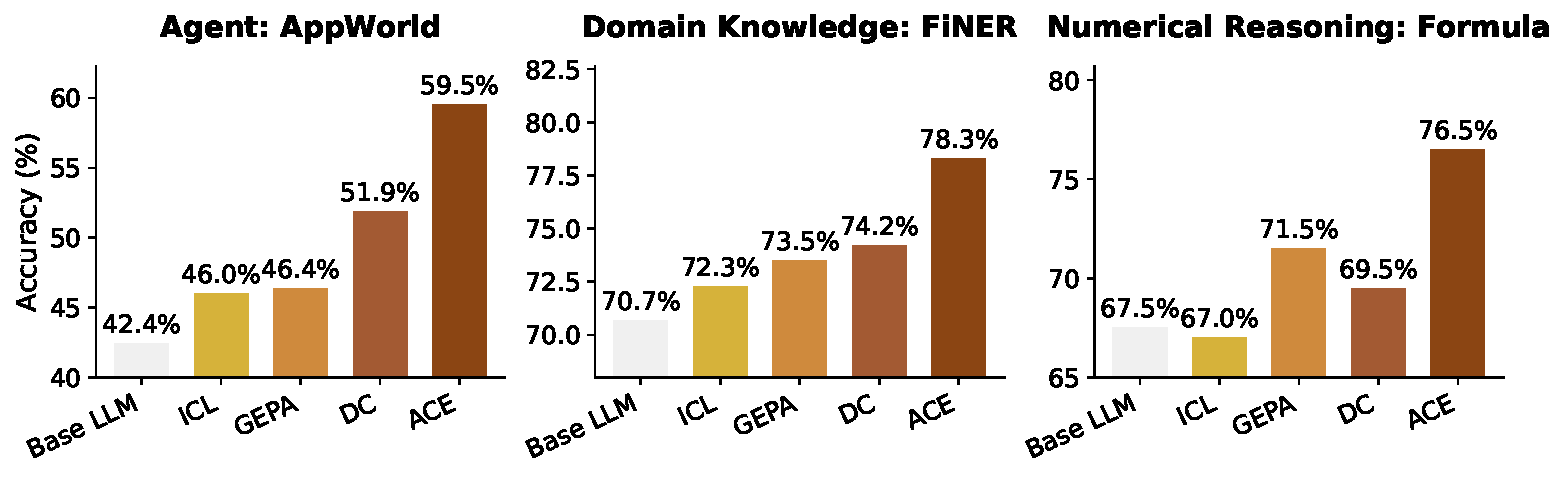
\includegraphics[width=0.95\textwidth]{figures/figure_1_CR.pdf}
    \caption{\textbf{Overall Performance Results.} Our proposed framework, ACE, consistently outperforms strong baselines across agent and domain-specific tasks.}
    \label{fig:overall-gain}
\end{figure}

Modern AI applications based on large language models (LLMs), such as LLM agents~\citep{yao2023react, yang2024swe} and compound AI systems~\citep{zaharia2024compoundGS}, increasingly depend on \textit{context adaptation}.
Instead of modifying model weights, context adaptation improves performance after model training by incorporating clarified instructions, structured reasoning steps, or domain-specific input formats directly into the model's inputs.
Contexts underpin many AI system components, including system prompts that guide downstream tasks~\citep{opsahl2024optimizing, agrawal2025gepa}, memory that carries past facts and experiences~\citep{suzgun2025dynamic, xu2025mem}, and factual evidence that reduces hallucination and supplements knowledge~\citep{asai2024self}.

Adapting through \textit{contexts} rather than \textit{weights} offers several key advantages.
Contexts are interpretable and explainable for users and developers~\citep{wei2022chain, wang2022self}, allow rapid integration of new knowledge at runtime~\citep{lewis2020retrieval, borgeaud2022improving}, and can be shared across models or modules in a compound system~\citep{khot2022decomposed}.
Meanwhile, advances in long-context LLMs~\citep{peng2023yarn} and context-efficient inference such as KV cache reuse~\citep{gim2024prompt, yao2025cacheblend} are making context-based approaches increasingly practical for deployment.
As a result, context adaptation is emerging as a central paradigm for building capable, scalable, and self-improving AI systems.

Despite this progress, existing approaches to context adaptation face two limitations.
First, \textit{brevity bias}: many prompt optimizers prioritize concise applicable instructions over comprehensive accumulation.
For example, GEPA~\citep{agrawal2025gepa} highlights brevity as a strength, but such abstraction can omit domain-specific heuristics, tool-use guidelines, or common failure modes that matter in practice~\citep{gao2025prompt}.
This objective aligns with validation metrics in some settings, but often fails to capture the detailed strategies required by agents and knowledge-intensive applications.
Second, \textit{context collapse}: methods that rely on monolithic rewriting by an LLM often degrade into shorter, less informative summaries over time, causing sharp performance declines (Figure \ref{fig:context-collapse}).
In domains such as interactive agents~\citep{trivedi2024appworld, patil2024gorilla, zhang2024caravan}, domain-specific programming~\citep{ye2023generating, zhang2025adaptive, zhang2025accelopt, mang2025frontiercs}, and financial or legal analysis~\citep{loukas2022finer, guha2023legalbench, wang2025finlora}, strong performance depends on retaining detailed, task-specific knowledge rather than compressing it away.

As applications like agents and knowledge-intensive reasoning demand greater reliability, recent work has shifted toward saturating contexts with abundant, potentially useful information~\citep{jiang2025putting, chung2025long, chen2025flora}, enabled by advances in long-context LLMs~\citep{peng2023yarn, mao2024lift}.
\textbf{We argue that contexts should function not as concise summaries, but as comprehensive, structured playbooks that are detailed, inclusive, and rich with domain insights.}
Unlike humans, who often benefit from concise generalization, LLMs are more effective when provided with long, detailed contexts and can distill relevance autonomously~\citep{jiang2025putting, liu2025selfelicit, suzgun2025dynamic}.
Thus, instead of compressing away domain-specific heuristics and tactics, contexts should preserve them, allowing the model to decide what matters during inference time.

To address these limitations, we introduce \name (\textbf{A}gentic \textbf{C}ontext \textbf{E}ngineering), a framework for comprehensive context adaptation in both offline settings (\eg system prompt optimization) and online settings (\eg test-time memory adaptation).
Rather than compressing contexts into distilled summaries, \name treats them as evolving playbooks that accumulate and organize strategies over time.
By design, \name incorporates a modular workflow of generation, reflection, and curation, while adding structured, incremental updates guided by a grow-and-refine principle.
This design preserves detailed, domain-specific knowledge, prevents context collapse, and yields contexts that remain comprehensive and scalable throughout adaptation.

We evaluate \name on two categories of LLM applications that most benefit from comprehensive, evolving contexts:
(1) \emph{agents}~\citep{trivedi2024appworld}, which require multi-turn reasoning, tool use, and environment interaction, where accumulated strategies can be reused across episodes; and
(2) \emph{domain-specific benchmarks}, which demand specialized tactics and knowledge, like financial analysis~\citep{loukas2022finer, wang2025finlora}.
Our key findings are:
\begin{packeditemize}
    \item \name consistently outperforms strong baselines, yielding average gains of 10.6\% on \textit{agents} and 8.6\% on \textit{domain-specific benchmarks}, across both offline and online adaptation settings.
    \item \name is able to construct effective contexts \textit{without} labeled supervision, instead leveraging execution feedback and environment signals, key ingredients for self-improving LLMs and agents.
    \item On the AppWorld benchmark leaderboard~\citep{AppWorldLeaderboard}, \name surpasses the top-1-ranked production-level agent IBM-CUGA~\citep{marreed2025towards} (powered by GPT-4.1) while using an open-source model (DeepSeek-V3.1).
    \item \name requires significantly fewer rollouts and achieves lower adaptation latency than existing adaptive methods, demonstrating that scalable self-improvement can be achieved with both higher accuracy and lower cost.
\end{packeditemize}